\documentclass[conference, compsoc, letterpaper]{IEEEtran}
\usepackage{graphicx}
\usepackage{subfig}
\usepackage{caption}
\usepackage{hyperref}
\usepackage{multirow}
 \usepackage[table,xcdraw]{xcolor}

\newcommand{\specialcell}[2][c]{\begin{tabular}[#1]{@{}c@{}}#2\end{tabular}}

\begin{document}

\title{Stars: Secure Shapes Based Challenge-Response User Authentication Protocols Against Passive Observers}
\author{\IEEEauthorblockN{Mohammad Amanzadeh\IEEEauthorrefmark{1}}
\IEEEauthorblockA{Department of Informatics}
\\
\IEEEauthorblockN{Constantine Roros\IEEEauthorrefmark{1}}
\IEEEauthorblockA{Department of Electrical and Computer Engineering}
\\
\IEEEauthorblockN{Sayed Hadi Hashemi\IEEEauthorrefmark{1}}
\IEEEauthorblockA{Department of Computer Science}
\\
\IEEEauthorblockA{\IEEEauthorrefmark{1}University of Illinois at Urbana-Champaign
\\\{amanzad2, roros2, hashemi3\}@illinois.edu}
}
\maketitle

\IEEEcompsoctitleabstractindextext{
	\begin{abstract}
	\boldmath
	When starting a new sport or practicing a new exercise program, it is extremely important to learn basic movements the right way, otherwise a long learning period or serious injuries are not unexpected. This highlights the importance of having a professional personal trainer. The problem is continuous access to such a person is expensive and not always possible.

This problem pushes the market to provide custom-designed sport gadgets. These gadgets are attached to the human body or accessories, then collect various data from built-in sensors. After that companion software analyze this data to evaluate the performance of the user.

Despite the promising outcome, there are some limitations that slow down the vast usage of these devices. First, these gadgets are still not affordable for everyone, and second their application is usually limited to one particular sport or even one particular movement, and can not be extended to others.

One way to overcome these limitations is to use more available devices for the training purposes.

In this work we propose a method to develop a personal trainer using common sensors of smartphone or health tracker. A Hidden Markov Model (HMM) has been trained for each action and classify the input motions by comparing the likelihood of HMMs trained on each action. We would also use a function of likelihood to assess the similarity of an action to the baseline. 
	\end{abstract}
}

\IEEEdisplaynotcompsoctitleabstractindextext
\IEEEpeerreviewmaketitle

\section{Introduction}
An important part of learning a new sport or exercise is understanding the right technique to correctly perform the physical activities involved. This ensures that people who engage in these activities do not get injured, get the most out of their work, and perform their best. In order to achieve such abilities, one usually hires a professional personal trainer. While this may be the best option, it is not the most affordable one. Many people have the desire and potential to learn new physical activities but may not have the resources or opportunity to work with a trainer. We hope that developing an application that helps people learn these activities will allow more people to better learn these activities by using a device (such as a smart watch or smart phone) that has an accelerometer. While these devices are not affordable for everyone, they are easier to access than a personal trainer.

The idea behind the application is that the person will wear the device as they are performing the physical activity. The application will indicate to the user what parts of the movement he or she needs to improve. If a user wears these devices while performing an activity, we can track that user’s movement using the accelerometer inside the device. In order to use this data to help the user train for a physical activity, there are a number of obstacles we must overcome. We must determine when the activity in question actually starts and ends during the accelerometer recording so we know what accelerometer features are specific to the actual activity. Once we figure out what features belong to each activity, we can use those features to classify the recording to figure out what activity the user is doing. In order to classify this data we developed a Hidden Markov Model for each activity by obtaining training data for each type of movement. Ideally the training data for these models is from accelerometer recordings of a user that is skilled at the given activity. Once we develop the model we can score the performance of the user when they complete the motion by comparing that motion to the recordings of the skilled user. Dynamic time warping is used to ensure that the different samples match up.




\section{Related Work}
Classification of human activities is a well-known machine learning problem. Work in \cite{Brand:1997wk} used HMM to classify complex activity. In this work, it is argued that simple HMM has the critical limitation of assuming the system, as a single process with a few states, therefore conventional HMM is not suitable for such detections. Therefore couple HMM is introduced in the work. \cite{Liu:2010cu} used accelerometer for gesture classification. In this method, raw input is quantitated before be used for training an HMM to classify gestures. 
An extension of human activity detection is to detect an activity in a stream. A study of Chambers et. al. in 2004 conducts a set of experiment to explorer and compare performance of different time series representations and distance measures \cite{Chambers:2004cu}. Later in 2008 Ding et. al. tried to segment sport activities using time series analysis. In their work they used HMM on a stream of accelerometer data to detect sport activities \cite{Ding:2008gq}.

\section{Motion Capture Process}
We have recorded 8 different activities (Table \ref{table-activities}). For each activity we did recordings on two different positions on the body: the arm (armband), and wrist (wristband). We used our right hand and right arm since we collected data from users that are right-handed. For each setting, 5 recordings were done to generate a total of 80 recordings. Since we currently do not have any professional trainers or athletes to obtain good data from, we recorded data using the partner who we felt was the most proficient at each activity. 

% Please add the following required packages to your document preamble:
% \usepackage{multirow}
\begin{table}[h]
\caption{List of Collected Activities}
\centering
\begin{tabular}{|l|l|}
\hline
\textbf{Sport}                        & \textbf{Activity} \\ \hline
\multirow{2}{*}{\textbf{Exercise}}   & Squat             \\ \cline{2-2} 
                                     & Press             \\ \hline
\multirow{3}{*}{\textbf{Basketball}} & Jump Shot         \\ \cline{2-2} 
                                     & One-Hand Pass     \\ \cline{2-2} 
                                     & Two-Hand Pass     \\ \hline
\multirow{3}{*}{\textbf{Tennis}}     & Forehand          \\ \cline{2-2} 
                                     & Backhand          \\ \cline{2-2} 
                                     & Serve             \\ \hline
\multirow{3}{*}{\textbf{Ping Pong}}  & Forehand          \\ \cline{2-2} 
                                     & Backhand          \\ \cline{2-2} 
                                     & Serve             \\ \hline
\end{tabular}
\label{table-activities}
\end{table}

Recordings collect a time series of various features from “iPhone 6” sensors (Table \ref{table-features})) at a rate of 100 frames per second. We used a smart phone to stream the data from the accelerometer through Wi-Fi to a computer where it was logged in a .csv file. We converted these .csv files to .mat files so we could analyze them in MATLAB.

\begin{table*}[h]
\label{table-features}
\caption{List of collected features in each recording}
\begin{tabular}{|l|p{3.5cm}|p{10.5cm}|}
\hline
\textbf{Category}               & \textbf{Feature}              & \textbf{Description} \\ \hline
\multirow{3}{*}{General}        & Time                           & Time at the beginning of the recording.                                                                    \\ \cline{2-3} 
                                & Time Stamp                     & Time as a long integer.                                                                                    \\ \cline{2-3} 
                                & Record Time                    & Time since recording.                                                                                      \\ \hline
\multirow{7}{*}{GPS}            & Coordination \{lat, long\}     & The geographical coordinate information.                                                                   \\ \cline{2-3} 
                                & Altitude                       & The altitude measured in meters.                                                                           \\ \cline{2-3} 
                                & Speed                          & The instantaneous speed of the device in meters per second.                                                \\ \cline{2-3} 
                                & Course                         & The direction in which the device is traveling.                                                            \\ \cline{2-3} 
                                & Vertical Accuracy              & The radius of uncertainty for the location, measured in meters.                                            \\ \cline{2-3} 
                                & Horizontal Accuracy            & The radius of uncertainty for the location, measured in meters.                                            \\ \cline{2-3} 
                                & Local Time Stamp               & The time at which this location was determined.                                                            \\ \hline
Accelerometer                   & Acceleration \{X,Y,Z\}         & The acceleration value for the \{x,y,z\} axis of the device.                                               \\ \hline
\multirow{4}{*}{Magnetometer}   & Heading \{X,Y,Z\}              & The geomagnetic data (measured in microteslas) for the \{x,y,z\}-axis.                                     \\ \cline{2-3} 
                                & True Heading                   & The heading (measured in degrees) relative to true north.                                                  \\ \cline{2-3} 
                                & Magnetic Heading               & The heading (measured in degrees) relative to magnetic north.                                              \\ \cline{2-3} 
                                & Heading Accuracy               & The maximum deviation (measured in degrees) between the reported heading and \newline the true geomagnetic heading. \\ \hline
Gyroscope                       & Motion Rotation Rate \{X,Y,Z\} & The rotation rate as measured by the device’s gyroscope.                                                   \\ \hline
\multirow{5}{*}{Pedometer}      & Activity                       & Getting the Type of Activity: stationary, walking, running, automotive, cycling, or unknown.               \\ \cline{2-3} 
                                & Activity Confidence            & The confidence that the motion data is accurate.                                                           \\ \cline{2-3} 
                                & Activity Start                 & The time at which the change in motion occurred.                                                           \\ \cline{2-3} 
                                & Steps                          & The number of steps taken by the user.                                                                     \\ \cline{2-3} 
                                & Last Step Date                 & The time at which steps are counted.                                                                       \\ \hline
\multirow{6}{*}{Processed Data} & Rotation \{X,Y,Z\}             & The rotation rate for each of the three axes in radians per second                                         \\ \cline{2-3} 
                                & Yaw                            & The yaw of the device, in radians.                                                                         \\ \cline{2-3} 
                                & Roll                           & The roll of the device, in radians.                                                                        \\ \cline{2-3} 
                                & Pitch                          & The pitch of the device, in radians.                                                                       \\ \cline{2-3} 
                                & User Acceleration \{X,Y,Z\}    & The acceleration that the user is giving to the device.                                                    \\ \cline{2-3} 
                                & Device Orientation             & The way user holds the device                                                                              \\ \hline
\end{tabular}
\end{table*}


\section{Method}
In order to determine if an action is performed correctly, we first need to identify the type of action. For that we first need to know what sport is playing at that moment and then search for the most likely action. Although this might be also possible to recognize action without knowing the kind of sport, however this makes the problem harder and will increase the response time. In addition we assume that when someone is playing a sport he will not change to another sport, and it should be convenient enough to ask the user to at least choose the kind of sport.

To recognize the actions we build a classifier for actions of each sport. The classifier is made with a Hidden Markov Model (HMM) for each action and recognizes a query action by comparing the likelihood of models. HMM assumes that a hidden process controls the probability of observing an event \cite{rabiner1986introduction}. The process has different hidden states and each state models a different distribution of data. In addition, the Markov property implies that the probability of being at a state at time $t$ only depends on the state of model at time $t-1$. The transitions of hidden states can have an ergodic architecture where the future state of model could be any of the $\{s_1,s_2,...,s_N\}$ states. Also we may use a left-right architecture and only allow auto-transition, and transition to the states with index greater than the current state.

In this work we use a left-right model that only allows auto-transition, and transition to the next state. This is convenient for recognizing sequences that follow a similar pattern and enforces the model to learn a continuous pattern over the action. We model the actions using HMMs with 4 hidden states. Each state models the movement features with a mixture of 2 Gaussians.

We use the data from gyroscope and accelerometer to construct the movement features. Gyroscope measures the rotation over the three axes which is a good feature for measuring the curvature of movement. The accelerometer measures the acceleration that is relative to the gravity, which is slightly different from the kinematic acceleration. An accelerometer in the rest position outputs $9.8$ on the axis that is flat to the ground, which is the gravity force. This will cause a low frequency on the axes of accelerometer that are pointed to the ground. By taking the derivative of acceleration, which is jerk, we can also filter out the low frequencies.

To recognize actions in real-time we need to consider different factors. First, the model should have a considerably low process time. Also we should be able to recognize actions without having information about the beginning and end frames of an action. Since we use a left-right architecture for the HMMs the processing time is linear and it needs $NT$ computations to identify the likelihood of an input action, where $N$ is the number of states of model and $T$ is the length of sequence. This is much faster than using an ergodic model which needs $N^2T$ processes.

We use a sliding window approach to recognize actions in real-time. With this method we segment the input data into parts with equal lengths of $32$ with $31$ frames overlap. For training the HMMs we use no overlap to avoid redundant samples. Since the data sampling rate is 100 frames per second 32 frames means about $\frac{1}{3}^{rd}$ of a second delay in output which is a good response time for our reason.

After the gesture recognition process, we need to identify the parts of an action that are not accurate. For this reason we proposed to find the similarity every frames of the action to a good sample of that action we have in the database. We use Dynamic Time Wrapping (DTW) to find the distance between the frames of a query action and the good sample of that action. With DTW we can find the closest match of a query frame on the sample in our dataset, and find the distance between the features at that point. For this analysis we use only the rotational features at this point of the research.

To identify the inaccurate parts with DTW, we need to have an entire sequence of an action. Therefore we should be able to tell an action from the transition parts between the consecutive actions and identify the beginning and ends respectively. For that we simplify the idea in \cite{lee1999hmm} and use an additional HMM to recognize non-action parts. We call this HMM the threshold model. We train the threshold HMM using all the samples of actions we have for a sport. This model should output a likelihood less than the likelihood of the action classifier for an action gesture. This is because the parameters of threshold HMM are trained on all the actions and it should be less certain than the correct model of an action. On the other hand the threshold model will output a likelihood higher than the other models on non-action sequences because of the large variance of its training data. 

\section{Results}
In this section we discuss the results of classification and error recognition of actions in table tennis. We trained an HMM for forehand, backhand, and serve actions using 10 samples in each dataset. Figure \ref{fig-viterbi} shows the 6 acceleration and rotation features and the most likely state sequence of each action using a sample in our test data.

By looking at the most likely hidden sequences we can tell that the classifiers divided the actions into 4 parts, where the beginning part is when the hand starts from rest. The second part is the preparation phase where the racket goes slightly back to prepare for hitting the ball. The third part is when it is moving towards the ball and the fourth part is when the hand goes back to rest. As we can see, the preparation phase in forehand and serve is longer than backhand. The reason is because in the backhand gesture the hand does not have enough space to prepare for hitting the ball, while in forehand and serve we have much more space.

Table \ref{table-score} shows the F1 score of recognizing the three gestures. Using the entire length of gestures for classification resulted in perfect classification. Using a sliding window also we had perfect recognition of the backhand and about $90\%$ accuracy in recognizing forehand and serve actions.

In a different experiment we also included the threshold HMM in the classifier to identify non-action parts. Table \ref{table-scoreThresh} shows the precision, recall, and F1 score of this test. As you can see, the precision of recognizing backhand and serve is 1, but for forehand and non-action gestures we received about $80\%$ precision. On the other hand the recall rate for non-action movement is 1. With this information we can tell that the classifier can perfectly recognize all the transition parts, but it sometimes classifies a non-action movement as forehand. 

One problem novice players have when starting table tennis is with the serve action. To have a good serve one should control the movement of the wrist and prevent it from bending. We collected examples of bending the hand when serving and experimented to see if we can recognize this error with DTW. Figure \ref{fig-distance} shows the distance matrix and the corresponding frames between a bad sample of the serve action and the good sample in our dataset. Also figure \ref{fig-good-bad} shows the comparison of the error rate of a bad sample and a good sample. As you can see on the bad serve sample, we get a very high error when the player hits the ball because of bending of the wrist. 

\begin{figure}
\centering
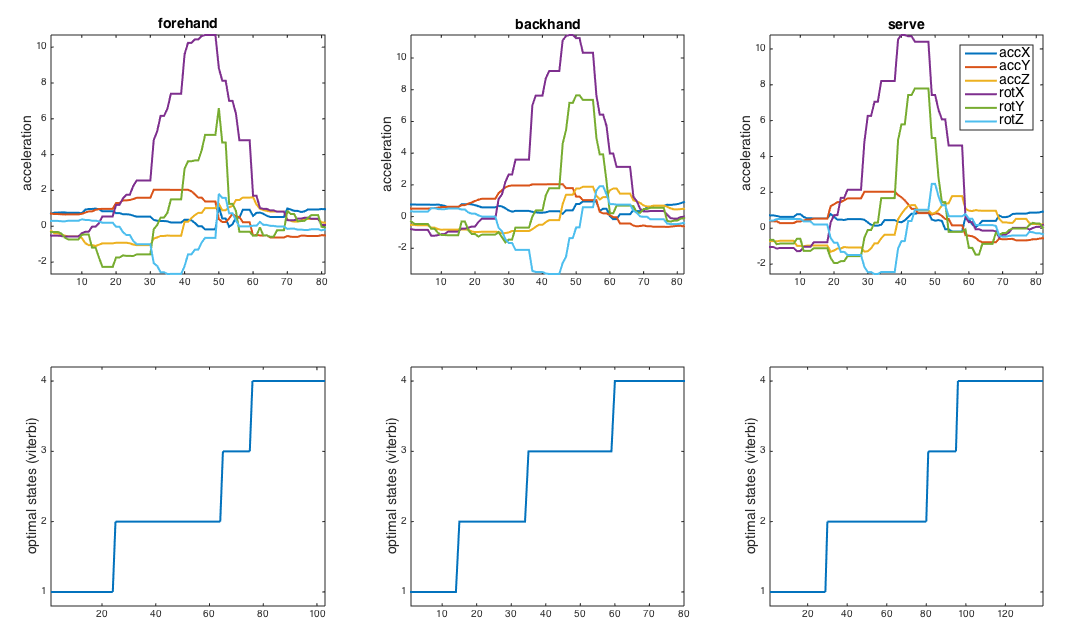
\includegraphics[width=3in]{resources/viterbi.png}
\caption{Most likely state sequence of a serve test action using Viterbi}
\label{fig-viterbi}
\end{figure}
\begin{table}[h]
\begin{tabular}{cccc}
                                        & \cellcolor[HTML]{C0C0C0}Forehand & \cellcolor[HTML]{C0C0C0}Backhand & \cellcolor[HTML]{C0C0C0}Serve \\
\cellcolor[HTML]{C0C0C0}entire sequence & 1.00                             & 1.00                             & 1.00                          \\
\cellcolor[HTML]{C0C0C0}window size 16  & 0.86                             & 0.89                             & 0.84                          \\
\cellcolor[HTML]{C0C0C0}window size 32  & 0.91                             & 1.00                             & 0.93                         
\end{tabular}
\caption{F1 score for recognizing each action using the whole gesture and sliding window of size 16 and 32 frames}
\label{table-score}
\end{table}
\begin{table}[h]
\begin{tabular}{ccccc}
                                  & \cellcolor[HTML]{C0C0C0}Forehand & \cellcolor[HTML]{C0C0C0}Backhand & \cellcolor[HTML]{C0C0C0}Serve & \cellcolor[HTML]{C0C0C0}Non-Gesture \\
\cellcolor[HTML]{C0C0C0}Precision & 0.84                             & 1.00                             & 1.00                          & 0.86                                \\
\cellcolor[HTML]{C0C0C0}Recall    & 0.92                             & 0.77                             & 0.78                          & 1.00                                \\
\cellcolor[HTML]{C0C0C0}F1 score  & 0.88                             & 0.87                             & 0.87                          & 0.92                               
\end{tabular}
\caption{Recognizing ping pong gestures from transition parts using a sliding window of size 32}
\label{table-scoreThresh}
\end{table}
\begin{figure}[tbp]
	\centering
	\subfloat[Good Serve]{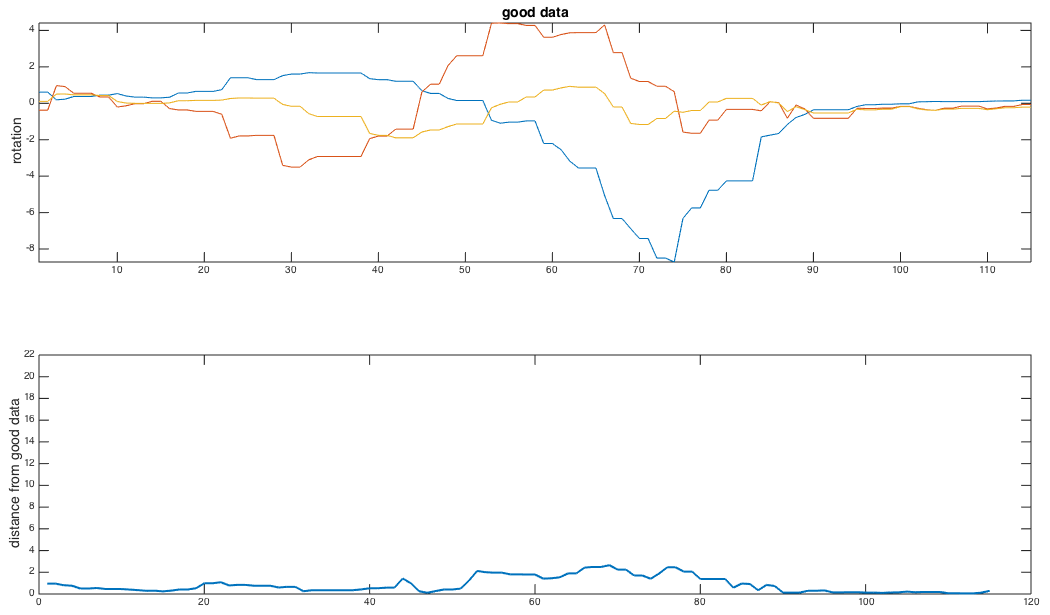
\includegraphics[width=3in]{resources/good.png}}\quad
	\subfloat[Bad Serve]{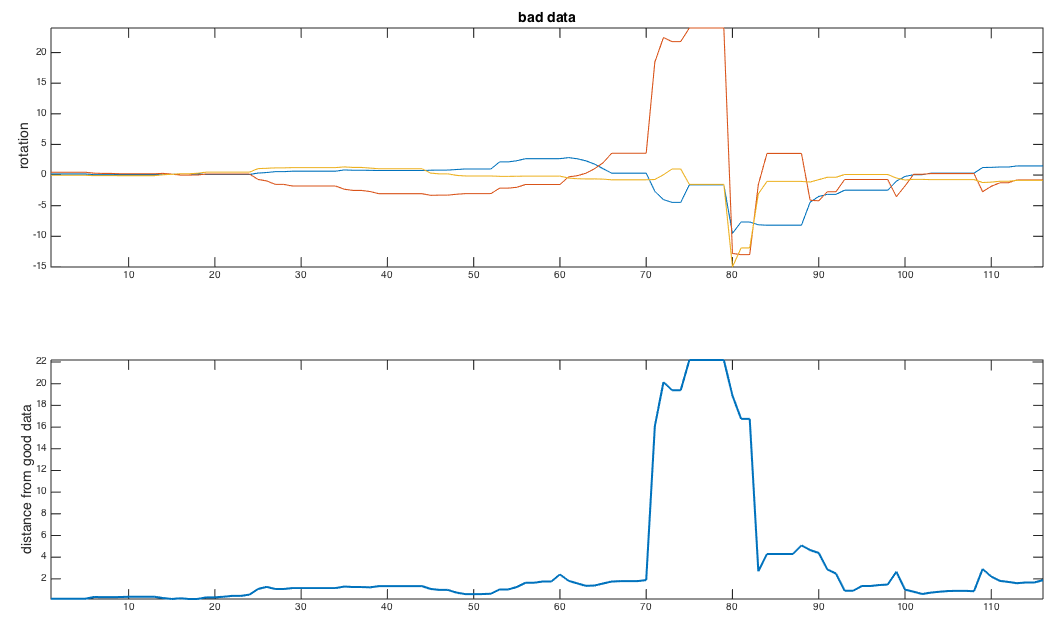
\includegraphics[width=3in]{resources/bad.png}}\\	
	\caption{3D rotation and error rate of a good and bad serve computed with DTW}
    \label{fig-good-bad}
\end{figure}
\begin{figure}
\centering
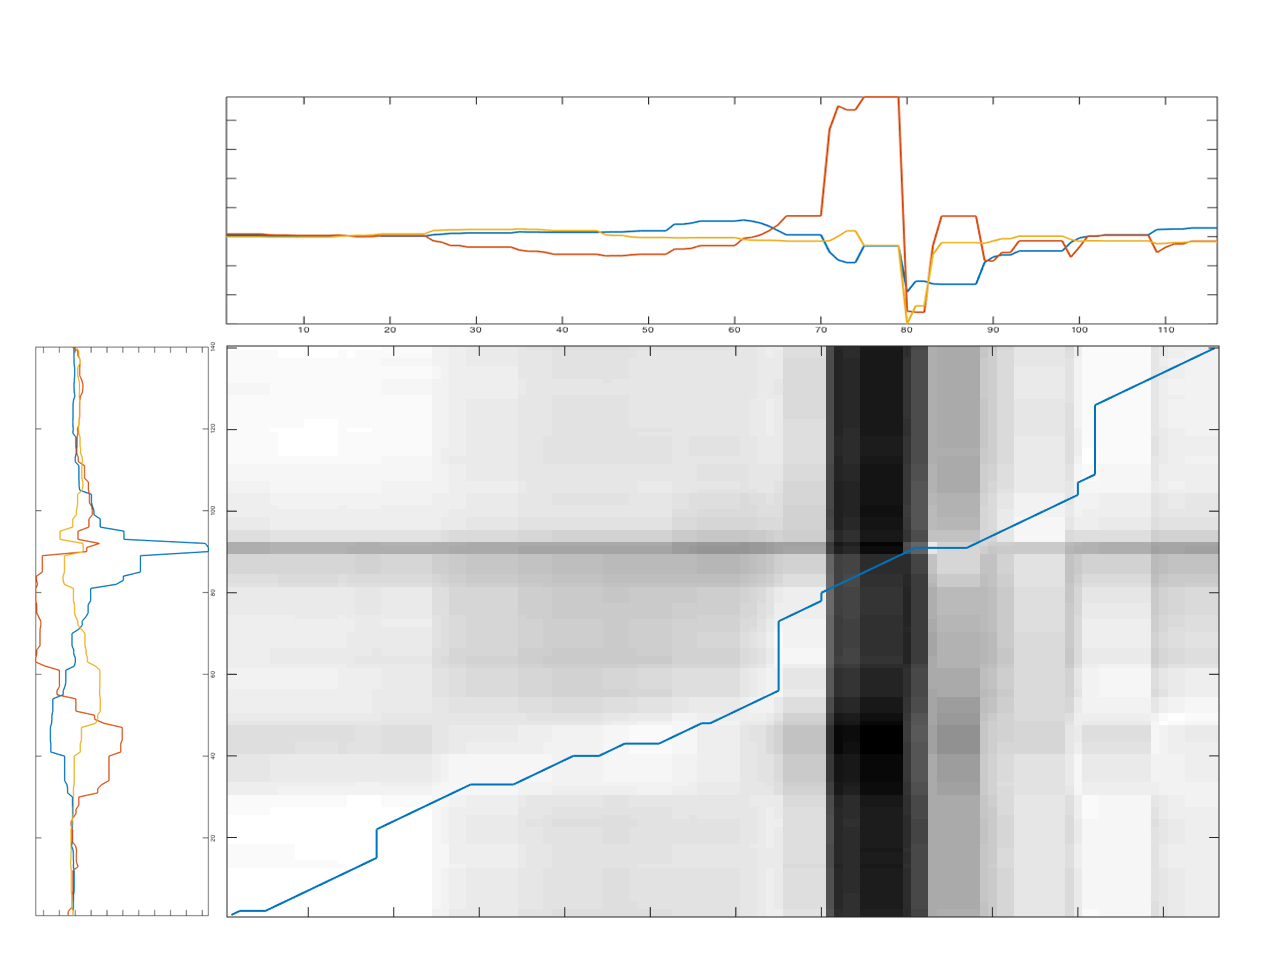
\includegraphics[width=3in]{resources/distance.jpg}
\caption{Distance between the 3 axes rotation of a good and bad serve}
\label{fig-distance}
\end{figure}


\section{Discussion and Future Work}
The goal of this system is to be able to run in real-time and help user to understand how good he performed an action. It also should provide a score to the accuracy of the entire session to help user understand how much he has improved. In addition we would like to provide a summary about the accuracy of performing each action and the parts of action that has the most error rate.

In order to notify user about the inaccurate parts in his performance we proposed that we can vibrate the cell phone when there is an error in some part of the action. Another possible approach is to show the places of error on the movement path. However we cannot measure the position using the phone sensors. A possible approach for constructing the movement trajectory from the mobile sensors is to use Kalman filter. \cite{sabatini2006quaternion} proposed a method with Kalman filters that can recognize the position using the accelerometer, gyroscope, and magnetometer.

Another issue of the current system is with the DTW algorithm. DTW needs $T^2$ computations, where $T$ is the length of a query gesture. This might cause problem when the length of a gesture is long. \cite{salvador2007toward} proposed a modified version of this algorithm that is able to process in $T$ computations and claimed that it is more accurate than the other methods for DTW. The FastDTW computes a subsample of a sequence with length $\sqrt{T}$ and by limiting the search space computes the distance in a time less than $T$. Then it projects the the estimated path from the subsampled sequence on the entire sequence and tries to estimate the correct points within a radius of frames around the estimated path.




\section{Conclusion}
We presented a system for real-time classification of sport gestures and identifying the inaccurate parts of the gestures. Our classification and error estimation process showed promising results in identifying the correct action and the erroneous frames of action. 

% \appendices
% \input{./sections/appendices.tex}

% \section*{Acknowledgments}
% The authors would like to thank\ldots

\ifCLASSOPTIONcaptionsoff
  \newpage
\fi

\bibliographystyle{apalike}
\bibliography{references}

\end{document}
 	